\documentclass[tikz, crop, margin=2mm]{standalone}

\begin{document}
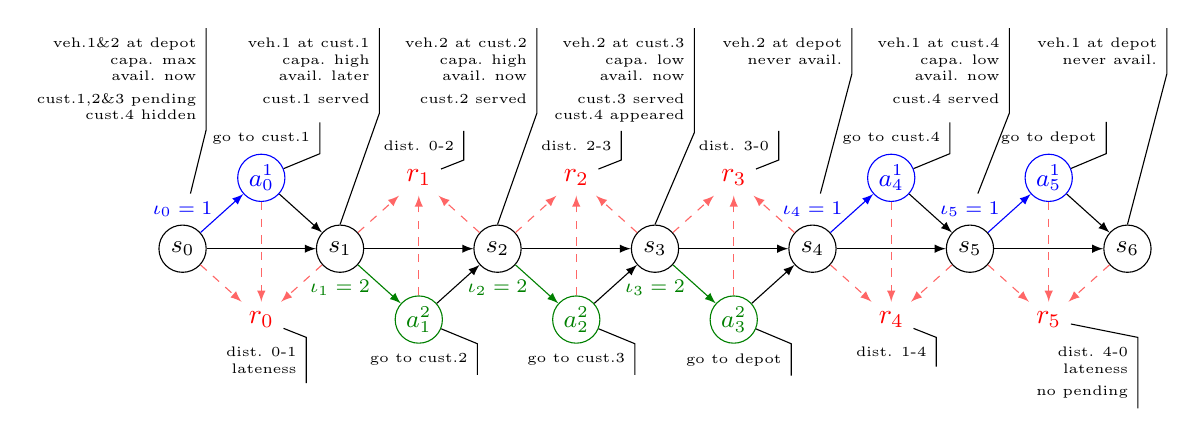
\begin{tikzpicture}[
    every node/.append style = {align = center},
    rand var/.style = {draw, circle, minimum width = 6mm, font=\small, inner sep=0.5mm},
    turn lbl/.style = {font=\scriptsize},
	var lbl/.style = {align=right, font=\tiny, anchor=north east},
    every path/.append style = {->, >=latex}
]

\foreach \t/\i in {0/1,1/2,2/2,3/2,4/1,5/1}{
    \node[rand var] (s\t) at (2*\t,0) {$s_\t$};
    \def\c{\ifnum\i=1{blue}\else{green!50!black}\fi}
    \node[rand var,\c] (a\i\t) at (2*\t+1,2.7-1.8*\i) {$a^\i_\t$};
	\node[turn lbl,\c] (i\t) at (2.*\t,1.5-\i) {$\iota_\t = \i$};
    \draw[\c] (s\t) -- (a\i\t);

	\node[red] (r\t) at (2*\t+1,1.8*\i-2.7) {$r_\t$};
}
\node[rand var] (s6) at (12,0) {$s_6$};
\foreach \t/\i/\n in {0/1/1,1/2/2,2/2/3,3/2/4,4/1/5,5/1/6}{
    \draw (s\t) -- (s\n);
    \draw (a\i\t) -- (s\n);

	\draw[red!60, dashed] (s\t) -- (r\t);
	\draw[red!60, dashed] (a\i\t) -- (r\t);
	\draw[red!60, dashed] (s\n) -- (r\t);
}

\def\toplbly{2.8}

\node[var lbl] (lbl) at (0.3,\toplbly)
	{veh.1\&2 at depot \\ capa. max \\ avail. now \\[1ex] cust.1,2\&3 pending \\ cust.4 hidden};
\draw[-] (0.1,0.7) -- (lbl.south east) -- (lbl.north east);

\node[var lbl, anchor=south] (lbl) at (a10.north) {go to cust.1};
\draw[-] (a10) -- (lbl.south east) -- (lbl.north east);

\node[var lbl] (lbl) at (2.5,\toplbly) {veh.1 at cust.1 \\ capa. high \\ avail. later \\[1ex] cust.1 served};
\draw[-] (s1.north) -- (lbl.south east) -- (lbl.north east);

\node[var lbl, anchor=north] (lbl) at (r0.south) {dist. 0-1 \\ lateness};
\draw[-] (r0) -- (lbl.north east) -- (lbl.south east);


\node[var lbl, anchor=north] (lbl) at (a21.south) {go to cust.2};
\draw[-] (a21) -- (lbl.north east) -- (lbl.south east);

\node[var lbl] (lbl) at (4.5,\toplbly) {veh.2 at cust.2 \\ capa. high \\ avail. now \\[1ex] cust.2 served};
\draw[-] (s2.north) -- (lbl.south east) -- (lbl.north east);

\node[var lbl, anchor=south] (lbl) at (r1.north) {dist. 0-2};
\draw[-] (r1) -- (lbl.south east) -- (lbl.north east);


\node[var lbl, anchor=north] (lbl) at (a22.south) {go to cust.3};
\draw[-] (a22) -- (lbl.north east) -- (lbl.south east);

\node[var lbl] (lbl) at (6.5,\toplbly)
	{veh.2 at cust.3 \\ capa. low \\ avail. now \\[1ex] cust.3 served \\ cust.4 appeared};
\draw[-] (s3.north) -- (lbl.south east) -- (lbl.north east);

\node[var lbl, anchor=south] (lbl) at (r2.north) {dist. 2-3};
\draw[-] (r2) -- (lbl.south east) -- (lbl.north east);


\node[var lbl, anchor=north] (lbl) at (a23.south) {go to depot};
\draw[-] (a23) -- (lbl.north east) -- (lbl.south east);

\node[var lbl] (lbl) at (8.5,\toplbly) {veh.2 at depot \\ never avail.};
\draw[-] (8.1,0.7) -- (lbl.south east) -- (lbl.north east);

\node[var lbl, anchor=south] (lbl) at (r3.north) {dist. 3-0};
\draw[-] (r3) -- (lbl.south east) -- (lbl.north east);


\node[var lbl, anchor=south] (lbl) at (a14.north) {go to cust.4};
\draw[-] (a14) -- (lbl.south east) -- (lbl.north east);

\node[var lbl] (lbl) at (10.5,\toplbly) {veh.1 at cust.4 \\ capa. low \\ avail. now \\[1ex] cust.4 served};
\draw[-] (10.1,0.7) -- (lbl.south east) -- (lbl.north east);

\node[var lbl, anchor=north] (lbl) at (r4.south) {dist. 1-4};
\draw[-] (r4) -- (lbl.north east) -- (lbl.south east);


\node[var lbl, anchor=south] (lbl) at (a15.north) {go to depot};
\draw[-] (a15) -- (lbl.south east) -- (lbl.north east);

\node[var lbl] (lbl) at (12.5,\toplbly) {veh.1 at depot \\ never avail.};
\draw[-] (s6.north) -- (lbl.south east) -- (lbl.north east);

\node[var lbl, anchor=north west] (lbl) at (r5.south west) {dist. 4-0 \\ lateness \\[1ex] no pending};
\draw[-] (r5) -- (lbl.north east) -- (lbl.south east);

\end{tikzpicture}
\end{document}
